\documentclass[10pt,letterpaper]{article} 
\usepackage{tabularx}
\usepackage{tikz}
\usepackage{toolsper}
%\usepackage{graphicx}‎‎
%\usefonttheme{serif}‎
%\usepackage{ptext}‎
%\usepackage{xepersian}
%\settextfont{B Nazanin}
\usepackage{lipsum}
\setlength{\parindent}{0pt}
\setlength{\parskip}{1em}
%\usepackage{enumitem}
%\setlist[enumerate,1]{label=(\arabic*)}
\newcommand{\pf}{$\blacksquare$}
\newcommand{\EX}{\Bbb E}
\newcommand{\nl}{\newline\newline}

\usepackage{amsmath}
\usepackage{accents}
\newlength{\dhatheight}
\newcommand{\doublehat}[1]{%
    \settoheight{\dhatheight}{\ensuremath{\hat{#1}}}%
    \addtolength{\dhatheight}{-0.35ex}%
    \hat{\vphantom{\rule{1pt}{\dhatheight}}%
    \smash{\hat{#1}}}}

\newcounter{QuestionNumber}
\setcounter{QuestionNumber}{1}

\newcommand{\Q}{
\textbf{
سوال \theQuestionNumber-
}
\stepcounter{QuestionNumber}
}

\newcommand{\fig}[3]{
\begin{figure}[h!]
#1
\caption{#2}
\label{#3}
\end{figure}
}

\newcommand{\subfig}[3]{
\begin{subfigure}{#3}
#1
\caption{#2}
\end{subfigure}
}

\newcommand{\figno}[1]{
\begin{figure}[h!]
#1
\end{figure}
}

\newcommand{\subfigno}[2]{
\begin{subfigure}{#2}
#1
\end{subfigure}
}
%\newcommand{\pic}[2]{
%\begin{center}
%\includegraphics[width=#2]{#1}
\newcommand{\testo}[5]{
\Q #1
\nl
1) #2
\nl
2) #3
\nl
3) #4
\nl
4) #5
\nl
}

\newcommand{\test}[5]{
\Q #1
\nl
{
\centering
%\begin{table}
%\begin{tabularx}{\linewidth}{r l X}
%\toprule
%1) #2\qquad\qquad & 2) #3\\ 
%3) #4\qquad\qquad & 4) #5\\
%\bottomrule
%\end{tabularx}
%\end{table}
\begin{tabularx}{0.8\textwidth} { 
   >{\raggedleft\arraybackslash}X 
%   >{\centering\arraybackslash}X 
   >{\raggedleft\arraybackslash}X  }
% \hline
1) #2\qquad\qquad\qquad\qquad & 2) #3\\ 
3) #4\qquad\qquad\qquad\qquad & 4) #5\\
%\hline
\end{tabularx}
%\begin{tabular}{\linewidth}{r c c}
%\end{tabular}
}
\nl
}




%\newcommand{\testo}[5]{
%\Q #1
%\nl
%{
%\centering
%\begin{tabular}{r c c}
%1) #2\qquad\qquad & 2) #3\\ 
%3) #4\qquad\qquad & 4) #5
%\end{tabular}
%}
%\nl
%}



%\newcommand{\testk}[5]{
%\Q #1
%\nl
%{
%\centering
%\begin{tabular}{r c c}
%1) #2\qquad\qquad\qquad\qquad & 2) #3\\ 
%3) #4\qquad\qquad\qquad\qquad & 4) #5
%\end{tabular}
%}
%\nl
%}
%\end{center}
%}
\begin{document}
\Large
\begin{center}
به نام زیبایی

سوالات پیشنهادی پایان ترم
\hl
\end{center}
\test{
کدام یک از سیگنال های زیر، تبدیل فوریه \underline{ندارد}؟
}
{$({1\over 2})^nu[n+1]$}
{$3^{n}u[-n+5]$}
{$(-4)^n u[n-3]$}
{$2^{n}\cdot{\sin \pi n}\cdot u[-n-1]$}
%%%%%%%%%%%%%%%%%%%%%%
\testo{
رابطه‌ی ورودی خروجی یک سیستم زمان گسسته به صورت زیر است:
$$
y[n]=(n-1)^2x[n-1]+x^*[n]
$$
رابطه‌ی ورودی خروجی این سیستم در حوزه‌ی فرکانس کدام است؟
}
{$Y(e^{j\omega})=-e^{-j\omega}{d X(e^{j\omega})\over d\omega}+X^*(e^{-j\omega})$}
{$Y(e^{j\omega})=-e^{-j\omega}{d^2 X(e^{j\omega})\over d\omega^2}+X^*(e^{-j\omega})$}
{$Y(e^{j\omega})=e^{j\omega}{d^2 X(e^{j\omega})\over d\omega^2}+X^*(e^{j\omega})$}
{$Y(e^{j\omega})=-e^{j\omega}{d^2 X(e^{j\omega})\over d\omega^2}+X^*(e^{j\omega})$}
%%%%%%%%%%%%%%%%%%%%%%
\test{
در شکل زیر، 
$
h_1[n]
$
حقیقی و 
$
H_1(e^{j\omega})=a_0+a_1e^{-j\omega}
$
است که در آن، 
$
a_0>0
$
 و 
$
H_1(e^{j\pi})=1
$
 می باشد. اگر 
$
h[n]
$
 پاسخ ضربه‌ی سیستم با ورودی 
$
x[n]
$
 و خروجی 
$
y[n]
$
به صورت زیر باشد:
\begin{figure}[h!]
\centering
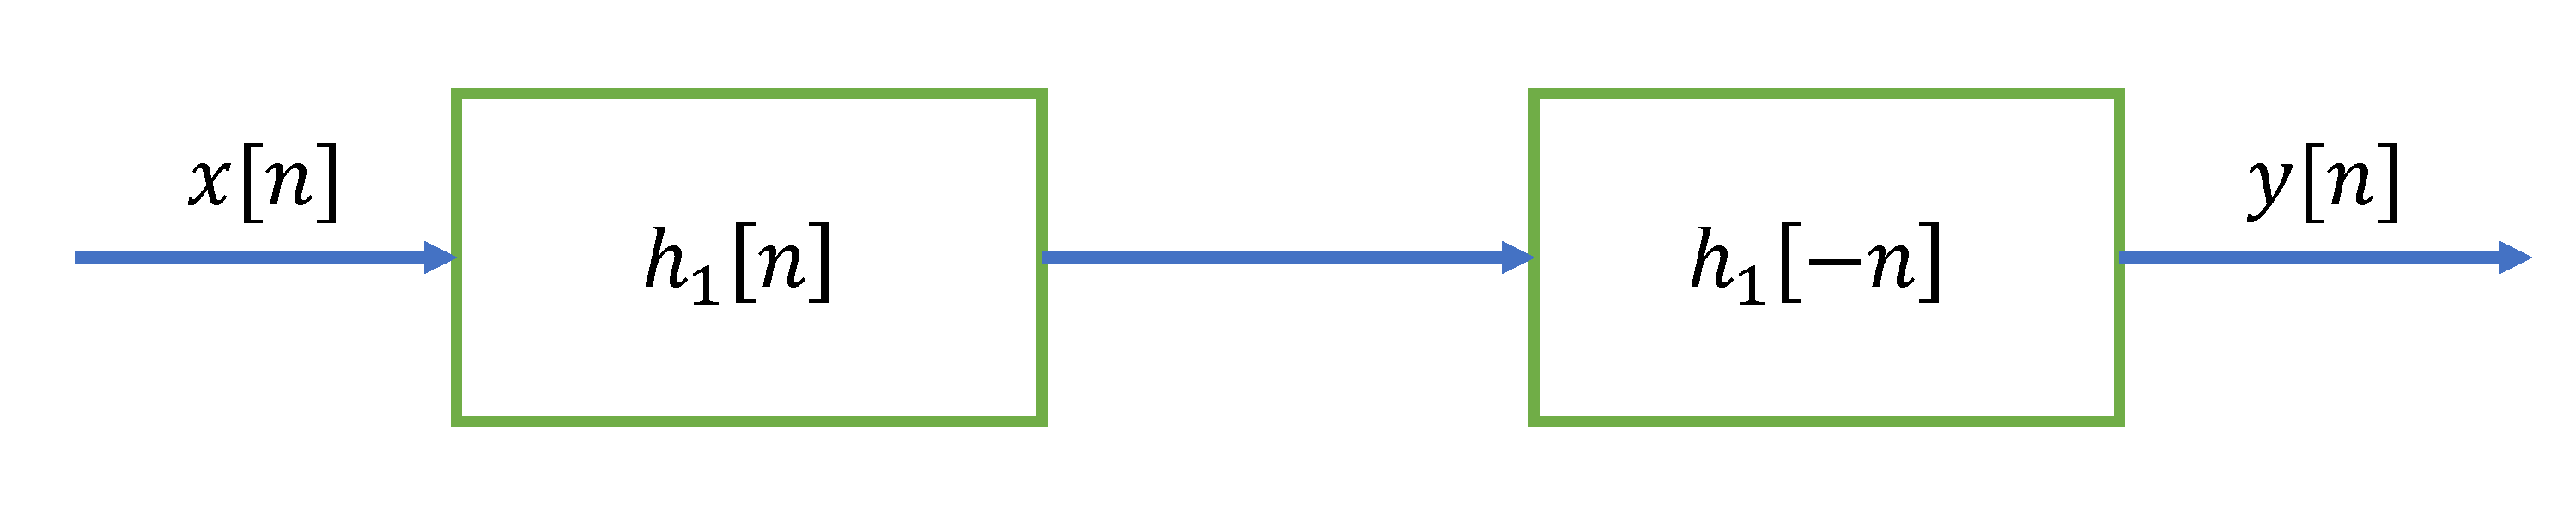
\includegraphics[width=100mm]{Q4_Final.pdf}
\end{figure}
$$
h[n]=\begin{cases}
13&,\quad n=0\\
6&,\quad n=\pm 1\\
0&,\quad \text{سایر جاها}\\
\end{cases}
$$
کدام گزینه درست است؟
}
{$a_0=2,a_1=1$}
{$a_0=3,a_1=2$}
{$a_0=2,a_1=-2$}
{$a_0=1,a_1=-1$}
%%%%%%%%%%%%%%%%%%%%%%
\test{
مقدار 
$
\int_{-\infty}^\infty \left|{dX(e^{j\omega})\over d\omega}\right|^2 d\omega
$
 برابر کدام گزینه است؟
}
{$\sum_{n=-\infty}^{\infty}|x[n]|^2$}
{$\sum_{n=-\infty}^{\infty}|x[n-1]|^2$}
{$\sum_{n=-\infty}^{\infty}n|x[n]|^2$}
{$\sum_{n=-\infty}^{\infty}n^2|x[n]|^2$}
%%%%%%%%%%%%%%%%%%%%%%
\test{
یک سیستم زمان گسسته را با ورودی 
$
x[n]
$
 و خروجی 
$
y[n]
$
در نظر بگیرید. تبدیل فوریه های ورودی و خروجی به صورت زیر به هم مرتبط هستند:
$$
Y(e^{j\omega})=\int_{\omega-{\pi\over 4}}^{\omega+{\pi\over 4}}X(e^{j\theta})e^{-j\theta}d\theta
$$
در این صورت، 
$
y[n]
$
 بر حسب 
$
x[n]
$
 کدام است؟
}
{$y[n]={2\over n}\sin\left({\pi\over 4}n\right)x[n-1]$}
{$y[n]={2\over n}\sin\left({\pi\over 4}n\right)x[n]$}
{$y[n]={2\over n}\sin\left({\pi\over 6}n\right)x[n]$}
{$y[n]={2j\over n}\sin\left({\pi\over 4}n\right)x[n+1]$}
%%%%%%%%%%%%%%%%%%%%%%
\test{
رابطه‌ی ورودی خروجی 5 سیستم زمان گسسته در حوزه‌ی فرکانس داده شده است:
$$
\begin{cases}
\text{سیستم 1}:  Y(e^{j\omega})=X(e^{2j\omega})\\
\text{سیستم 2}:  Y(e^{j\omega})={1\over 1-e^{-j\omega}}X(e^{j\omega})+\pi X(e^{j0})\sum_{k=-\infty}^{\infty}\delta(\omega-2\pi k)\\
\text{سیستم 3}:  Y(e^{j\omega})=e^{3j\omega}X(e^{j\omega})\\
\text{سیستم 4}:  Y(e^{j\omega})={d\over d\omega}X(e^{j\omega})\\
\text{سیستم 5}:  Y(e^{j\omega})={1\over2\pi}\int_{0}^{2\pi}X(e^{j\theta})X(e^{j(\omega-\theta)})d\theta\\
\end{cases}
$$
چندتا از این سیستم ها خطی و تغییر ناپذیر با زمان هستد؟
}
{1}
{2}
{3}
{4}
%%%%%%%%%%%%%%%%%%%%%%
\testo{
فرض کنید اطلاعات زیر برای یک سیگنال حقیقی $x[n]$ با تبدیل فوریه‌ی $X(e^{j\omega})$ داده شده اند:

1. $x[n]=0\quad,\quad n>0$

2. $x[0]>0$

3. $\Im\{X(e^{j\omega})\}=\sin \omega-\sin 2\omega$

4. ${1\over 2\pi}\int_0^{2\pi}|X(e^{j\omega})|^2 d\omega=3$

در این صورت، سیگنال $x[n]$ کدام است؟
}
{$\delta[n]-\delta[n-1]$}
{${1\over 2}\delta[n]+{1\over 2}\delta[n+1]-{1\over 2}\delta[n+2]$}
{$\delta[n]+\delta[n+1]-\delta[n+2]$}
{$\delta[n]+\delta[n-1]-\delta[n-2]$}
%%%%%%%%%%%%%%%%%%%%%%
\test{
یک سیستم زمان گسسته با پاسخ فرکانسی داده شده در شکل زیر مفروض است. خروجی این سیستم به ازای ورودی 
$
x[n]=\sum_{k=-\infty}^{\infty}(-1)^k\delta[n-2k]
$
 برابر کدام است؟
\begin{figure}[h!]
\centering
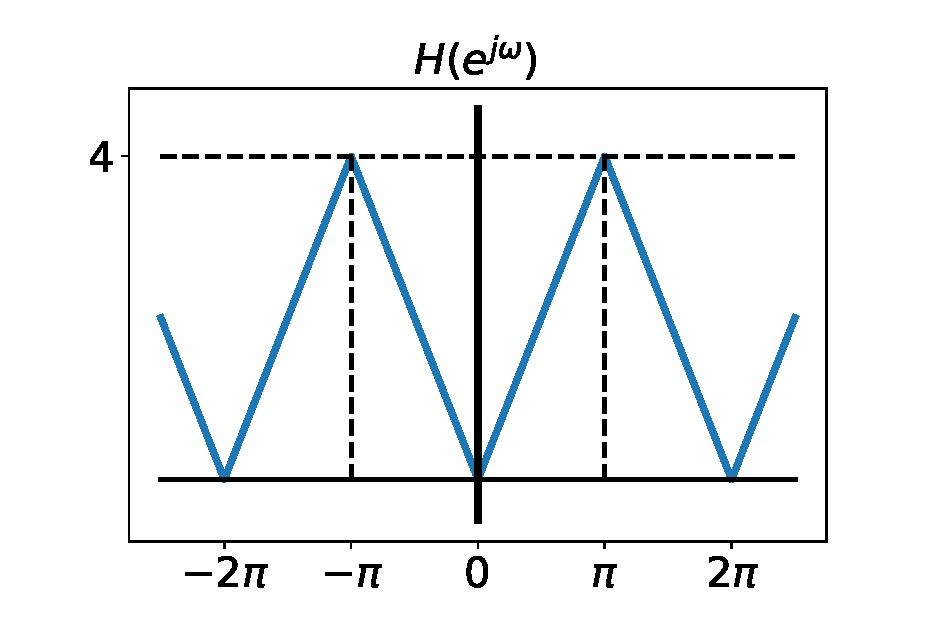
\includegraphics[width=80mm]{Q8_Final}
\end{figure}
}
{$2(-1)^n+2\cos({\pi\over 2}n)$}
{$(-1)^n+\cos({\pi\over 2}n)$}
{$\cos({\pi\over 2}n)$}
{$2\cos({\pi\over 2}n)$}
%%%%%%%%%%%%%%%%%%%%%%
\test{
برای کدام یک از سیگنال های $x[n]$ زیر با تبدیل فوریه‌ی 
$
X(e^{j\omega})
$
 داریم 
$$
\int_0^{2\pi} {dX(e^{j\omega})\over d\omega}e^{j\omega} d\omega=0
$$
؟
}
{$x[n]=\delta[n-1]+{\sin \pi n\over \pi (n-{1\over 2})}$}
{$x[n]=({1\over 3})^nu[n]$}
{$x[n]=2^n u[-4-n]$}
{$x[n]=u[n]$}
%%%%%%%%%%%%%%%%%%%%%%
\test{
یک سیستم زمان گسسته دارای ورودی 
$
x[n]
$
 و خروجی 
$
y[n]
$
است. تبدیل فوریه های ورودی و خروجی با رابطه‌ی زیر به هم مربوط می شوند:
$$
Y(e^{j\omega})=2X(e^{j\omega})+3e^{-j\omega}X(e^{j\omega})+5j{d X(e^{j\omega})\over d\omega}
$$
کدام گزینه در مورد این سیستم درست است؟
}
{غیرخطی است.}
{پایدار است.}
{علی است.}
{تغییر ناپذیر با زمان است.}
%%%%%%%%%%%%%%%%%%%%%%
\textbf{سوالات تشریحی}

\vspace{5mm}

\Q
ورودی 
$
x[n]=({1\over 2})^n u[n]
$
 به سیستمی با پاسخ فرکانسی
$
H(e^{j\omega})={1\over (1-{1\over 2}e^{-j\omega})(1-{1\over 3}e^{-j\omega})}
$
 وارد می‌شود. رابطه‌ی زمانی خروجی را بیابید.

\Q 
برای سیگنال زمانی $x[n]$ زیر با تبدیل فوریه‌ی 
$
X(e^{j\omega})
$
، هر یک از موارد الف) تا ت) را بیابید.

\begin{figure}[h!]
\centering
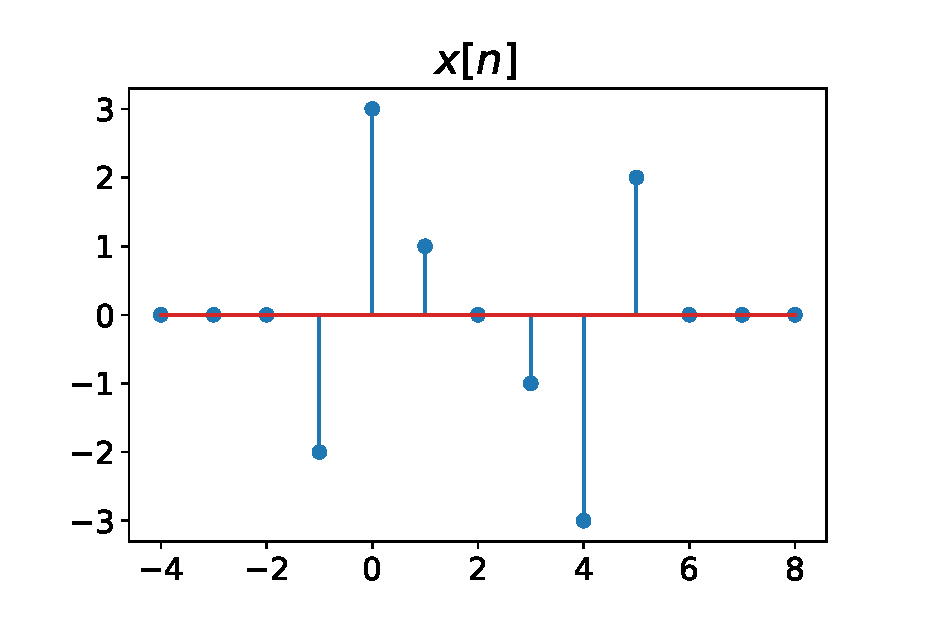
\includegraphics[width=80mm]{Q12_Final.eps}
\end{figure}

الف)
$
X(e^{j0})
$

ب)
$
X(e^{j\pi})
$

پ)
$
\measuredangle X(e^{j\omega})
$

ت)
$
{1\over 2\pi}\int_0^{2\pi} \left|{d X(e^{j\omega})\over d \omega}\right|^2d\omega
$

\Q
یک سیستم زمان گسسته‌ی پایدار و علی دارای این خاصیت است که
$$
({4\over 5})^u[n]\to n({4\over 5})^u[n]
$$
در این صورت، پاسخ فرکانسی این سیستم را بیابید.

\Q
 یک سیستم با رابطه ورودی خروجی زیر مفروض است:
$$
y[n]+{1\over 2}y[n-1]=x[n]
$$
 پاسخ این سیستم به ورودی های زیر چیست؟

الف)
$
x[n]=(-{1\over 2})^nu[n]
$

ب)
$
x[n]=\delta[n]+{1\over 2}\delta[n-1]
$

\Q
اگر سیگنال 
$
x[n]
$
 دارای تبدیل فوریه‌ی 
$
X(e^{j\omega})
$
باشد، تبدیل فوریه‌ی هر یک از سیگنالهای زیر را بر حسب 
$
X(e^{j\omega})
$
بنویسید ($x[n]$ الزاما حقیقی نیست).

الف)
$
y[n]=nx^*[-n]
$

ب)
$
y[n]=\Re\{x[n+1]\}
$
%\test{
%$
%\delta(t^2-1)
%$
%برابر کدام گزینه است؟
%}
%{
%$
%\delta(t-1)+\delta(t+1)
%$
%}
%{
%$
%\delta(t-1)-\delta(t+1)
%$
%}
%{
%$
%{1\over 2}\delta(t-1)-{1\over 2}\delta(t+1)
%$
%}
%{
%$
%{1\over 2}\delta(t-1)+{1\over 2}\delta(t+1)
%$
%}
%\testo{
%سیستم کلی با ورودی x[n] و خروجی y[n] را به صورت شکل زیر در نظر بگیرید که در آن، رابطه‌ی ورودی-خروجی هر سیستم به صورت زیر است:
%\qn{
%&\text{سیستم 1}:\quad y[n]=\begin{cases}x[n/2]&,\quad \text{n زوج}\\0&,\quad \text{n فرد}\end{cases}
%\\&\text{سیستم 2}:\quad y[n]=x[n]+{1\over 2}x[n-1]+{1\over 4}x[n-2]
%\\&\text{سیستم 3}:\quad y[n]=x[2n]
%}{}
%کدام گزینه رابطه‌ی ورودی خروجی سیستم زیر را بدرستی نشان می دهد؟
%\begin{figure}[h!]
%\centering
%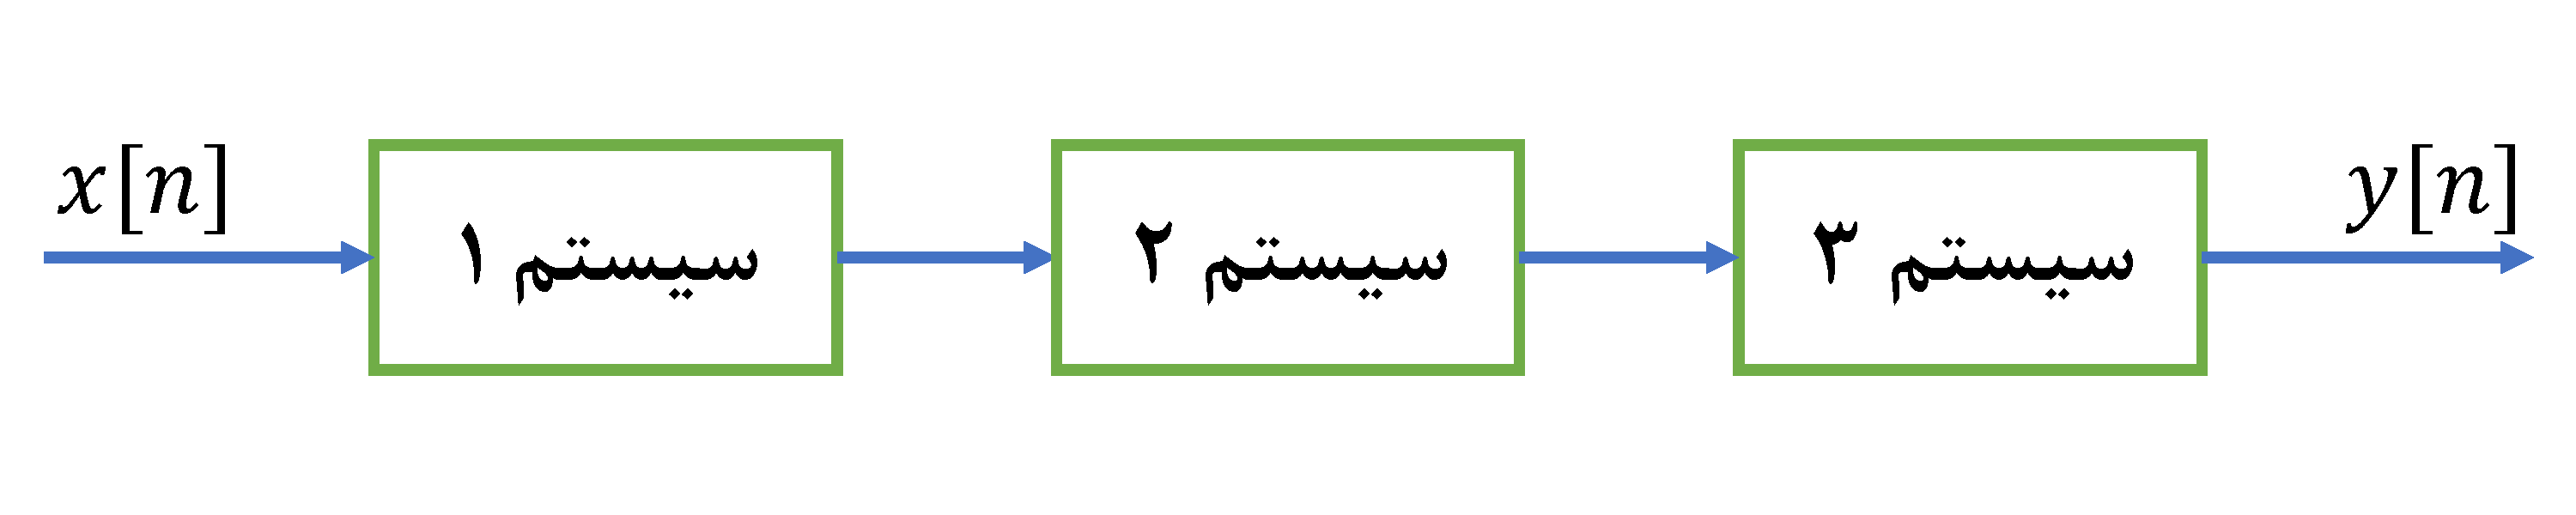
\includegraphics[width=120mm]{_2Q.pdf}
%\end{figure}
%}
%{
%$y[n]=\begin{cases}x[n]+{1\over 2}x[n-1]+{1\over 4}x[n-2]&,\quad \text{n زوج}\\0&,\quad \text{n فرد}\end{cases}$
%}
%{
%$y[n]=\begin{cases}x[n]+{1\over 2}x[n-2]+{1\over 4}x[n-4]&,\quad \text{n زوج}\\0&,\quad \text{n فرد}\end{cases}$
%}
%{$y[n]=x[n]+{1\over 4}x[n-1]$}
%{$y[n]=x[n]+{1\over 2}x[n-1]+{1\over 4}x[n-2]$}
%%%%%%%%%%%%%%%%%%%%%%%%%
%\test{
%مقدار انتگرال 
%$
%I=\int_{-\infty}^\infty X^2(j\omega)d\omega
%$
% برای سیگنال زیر کدام است؟
%\begin{figure}[h!]
%\centering
%\includegraphics[width=70mm]{_3Q.eps}
%\end{figure}
%}
%{$\pi$}
%{$2\pi$}
%{$1\over 2$}
%{1}
%%%%%%%%%%%%%%%%%%%%%%%%
%\newpage
%\test{
%یک سیستم با رابطه‌ی ورودی-خروجی 
%$
%y[n]=\cos \left({\pi\over 2}x[n]\right)
%$
%داده شده است. کدام گزینه در مورد متناوب بودن خروجی به ازای 
%$
%x[n]={n^2\over 4}
%$
%صحیح است؟
%}
%{متناوب با فرکانس اصلی $\pi\over 3$ است.}
%{متناوب با فرکانس اصلی $\pi\over 4$ است.}
%{متناوب با فرکانس اصلی $\pi\over 8$ است.}
%{متناوب نیست.}
%%%%%%%%%%%%%%%%%%%%%%%%%
%\test{
%در یک سیستم LTI زمان گسسته با پاسخ ضربه‌ی 
%$
%h[n]=({1\over 2})^{|n|}
%$
%، 
%پاسخ به ورودی 
%$
%x[n]=u[n]+u[2-n]
%$
% در لحظه‌ی 
%$
%n=-2
%$
%کدام است؟ ($u[n]$ تابع پله‌ی واحد است)
%}
%{$31\over 8$}
%{$55\over 16$}
%{$19\over 4$}
%{4}
%%%%%%%%%%%%%%%%%%%%%%%%%%%%
%\test{
%تبدیل فوریه‌ی سیگنال $x(t)$ به شکل زیر است. کدام مورد در مورد این سیگنال صحیح است؟
%\begin{figure}[h!]
%\centering
%\includegraphics[width=70mm]{_6Q.eps}
%\end{figure}
%}
%{$\angle x(t)=t$}
%{$x(t)$ حقیقی است.}
%{$\angle x(t)=-t$}
%{$x(t)$ موهومی و زوج است.}
%%%%%%%%%%%%%%%%%%%%%%%%%%%%%%
%\test{
%سیگنال $x(t)$ را با تبدیل فوریه‌ی 
%$
%X(j\omega)
%$
% در نظر بگیرید. فرض کنید اطلاعات زیر را در مورد سیگنال 
%$
%x(t)
%$
% داریم:
%\nl
%$\blacksquare$
% سیگنال $x(t)$ حقیقی است.
%
%$\blacksquare$
%$x(t)=0\quad,\quad t\le 0$
%
%$\blacksquare$
%$\int_{-\infty}^\infty \Re\{X(j\omega)\}e^{j\omega t}d\omega=2\pi |t|e^{-|t|}$
%\nl
%$x(t)$
% برابر کدام است؟
%}
%{$2\pi te^{-t}u(t)$}
%{$2\pi te^{t}u(t)$}
%{$2te^{t}u(t)$}
%{$2te^{-t}u(t)$}
%%%%%%%%%%%%%%%%%%%%%%%%%%%%%%
%\test{
%حاصل کانولوشن 
%$
%{\sin^2\pi t\over \pi^2t^2}*\cos^2{\pi t\over 2}
%$
% برابر کدام است؟
%
%(یادآوری:
%$
%\Pi\left({t\over 2T}\right)\iff 2T\text{sinc}\left({\omega T\over \pi}\right)
%$
%)
%}
%{$0.25+0.5\cos^2{\pi t\over 2}$}
%{$-0.25+0.5\cos^2{\pi t\over 2}$}
%{$\cos^2{\pi t\over 2}$}
%{$0.5\cos^2{\pi t\over 2}$}
%%%%%%%%%%%%%%%%%%%%%%%%%%%
%\test{
%رابطه‌ی ورودی-خروجی برای 4 سیستم به صورت زیر است:
%\qn{
%&\text{سیستم 1}: 
%y(t)=\begin{cases}
%0&,\quad x(t)<0\\
%x(t)+x(t-2)&,\quad x(t)\ge 0
%\end{cases}
%\\&\text{سیستم 2}: 
%y(t)=\begin{cases}
%0&,\quad t<0\\
%x(t)+x(t-2)&,\quad t\ge 0
%\end{cases}
%\\&\text{سیستم 3}: y(t)=\int_{-\infty}^{2t}x(\tau)d\tau
%\\&\text{سیستم 4}: y(t)=x(t-2)+x(2-t)
%}{}
%کدام سیستم در خاصیت تغییرپذیری با زمان از بقیه متفاوت است؟
%}
%{1}
%{2}
%{3}
%{4}
%%%%%%%%%%%%%%%%%%%%%%%%%%
%\test{
%اگر توصیف ورودی خروجی یک سیستم به صورت 
%$
%y(t)=x(-t)+2
%$
% باشد، رابطه ی ورودی-خروجی وارون آن برابر کدام است؟
%}
%{$y(t)=x(t)-2$}
%{$y(t)=x(-t)-2$}
%{$y(t)=x(-t)+2$}
%{$y(t)=x(t)+2$}
%%%%%%%%%%%%%%%%%%%%%%%%%%%
%\test{
%سیگنالی داریم که دارای تبدیل فوریه‌ی 
%$$
%X(j\omega)=j\sqrt\pi \text{sgn}(\omega)[u(\omega+1)-u(\omega-1)]
%$$
% است. مقدار مشتق این سیگنال در $t=0$ چقدر است؟
%}
%{$-{\sqrt\pi\over 2}$}
%{$-{1\over\sqrt\pi}$}
%{0}
%{$-{1\over 2\sqrt\pi}$}
%%%%%%%%%%%%%%%%%%%%%%%%%%%%
%\testo{
%$
%x_1(t)
%$
% متناوب با پریود اصلی
%$
%T_1$
% و ضرایب سری فوریه‌ی 
%$
%a_k
%$
% و 
%$
%x_2(t)
%$
% متناوب با پریود اصلی
%$
%T_2=3T_1
%$ و ضرایب سری فوریه‌ی 
%$
%b_k
%$
%است. ضرایب سری فوریه‌ی 
%$
%y(t)=x_1(t)+x_2(t)
%$
% کدام است؟
%}
%{
%$
%\begin{cases}
%a_{n\over 3}+b_n&,\quad \text{اگر n مضرب 3 باشد}
%\\b_n&,\quad \text{در غیر این صورت}
%\end{cases}
%$
%}
%{
%$
%\begin{cases}
%a_{n\over 3}+b_n&,\quad \text{اگر n مضرب 3 باشد}
%\\a_n&,\quad \text{در غیر این صورت}
%\end{cases}
%$
%}
%{
%$
%\begin{cases}
%b_n+b_{n\over 3}&,\quad \text{اگر n مضرب 3 باشد}
%\\b_n&,\quad \text{در غیر این صورت}
%\end{cases}
%$
%}
%{
%$
%\begin{cases}
%a_n+b_{n\over 3}&,\quad \text{اگر n مضرب 3 باشد}
%\\a_n&,\quad \text{در غیر این صورت}
%\end{cases}
%$
%}
%%%%%%%%%%%%%%%%%%%%%%%
%\test{
%رابطه‌ی 
%$
%x(t)*x(t)=3x\left({t\over 2}\right)
%$
% برای کدام یک از سیگنال های زیر برقرار است؟ (منظور از * عملگر کانولوشن است)
%}
%{$3\over \pi^2+t^2$}
%{${3\over \pi}{1\over 5-jt}$}
%{$6{\sin\pi t\over \pi t}$}
%{$3\pi \delta({t\over 2}-1)$}
%%%%%%%%%%%%%%%%%%%%%%%%%
%\test{
%با اعمال کدام یک از ورودی‌های زیر به یک سیستم LTI و مشاهده‌ی خروجی، می توان پاسخ ضربه‌ی آن سیستم را به طور یکتا بدست آورد؟
%}
%{${\sin^2 \pi t\over \pi t}$}
%{$\Pi(t)$}
%{$u(t)$}
%{$\cos 2t$}
%%%%%%%%%%%%%%%%%%%%%%%%%%%%
%\test{
%سیستم LTI ای با پاسخ ضربه‌ی 
%$
%h(t)={\sin(4(t-1))\over \pi(t-1)}
%$
% را در نظر بگیرید. پاسخ این سیستم به ورودی 
%$
%x(t)=\left[{\sin (2t)\over \pi t}\right]^2
%$
% کدام است؟
%}
%{
%$
%{\sin(2(t-1))\over \pi(t-1)}
%\times
%{\sin(2(t-{1\over 2}))\over \pi(t-{1\over 2})}
%$
%}
%{$\left[{\sin (2(t-1))\over \pi (t-1)}\right]^2$}
%{$\left[{\sin (4(t-1))\over \pi (t-1)}\right]^2$}
%{$\left[{\sin (2(t-{1\over 2}))\over \pi (t-{1\over 2})}\right]^2$}
%%%%%%%%%%%%%%%%%%%%%%%%%%%%%%
%\test{
%مقدار 
%$
%\sum_{k=-\infty}^{\infty}{\sin^2({k\pi\over 2})\over k^2}
%$
%برابر کدام است؟
%}
%{$\pi^2\over 2$}
%{$\pi^2$}
%{$\pi\over 2$}
%{$1\over 2$}
%%%%%%%%%%%%%%%%%%%%%%%%%%%%%%%
%\test{
%سیگنال متناوب نشان داده شده در شکل زیر، از سیستمی با پاسخ ضربه‌ی 
%$
%h(t)={\sin({\pi\over 2}t)\over \pi t}
%$
% عبور می کند. سیگنال خروجی برابر کدام است؟
%\begin{figure}[h!]
%\centering
%\includegraphics[width=70mm]{_17Q.eps}
%\end{figure}
%}
%{$-{2\over \pi}\sin({\pi\over 3}t)$}
%{${2\pi}\cos({\pi\over 3}t)$}
%{${2\over \pi}\sin({\pi\over 6}t)$}
%{${3\over 2\pi}\cos({\pi\over 3}t)$}
%%%%%%%%%%%%%%%%%%%%%%%%%%%%%%%%%
%\test{
%سیگنال متناوب $x(t)$ با ضرایب سری فوریه‌ی زیر مفروض است:
%$$
%c_k=\begin{cases}
%1&,\quad k=0
%\\
%-j\left({1\over 3}\right)^{|k|}&,\quad k\ne0
%\end{cases}
%$$
%کدام گزینه در مورد این سیگنال درست است؟
%}
%{سیگنال $x(t)$ حقیقی است.}
%{سیگنال $x(t)$ فرد است.}
%{مشتق سیگنال $x(t)$ زوج است.}
%{مشتق سیگنال $x(t)$ فرد است.}
%%%%%%%%%%%%%%%%%%%%%%%%%%%%%%%%%%%
%\test{
%رابطه‌ی بین ورودی و خروجی یک سیستم زمان گسسته به صورت زیر است:
%$$
%y[n]=\begin{cases}
%\Re\{x[n-1]\}&,\quad \text{n زوج}
%\\\Re\{x[n-1]+x[n-2]\}&,\quad \text{n فرد}
%\end{cases}
%$$
%کدام گزینه در مورد این سیستم درست است؟
%}
%{خطی و تغییر ناپذیر با زمان}
%{خطی و تغییر پذیر با زمان}
%{غیرخطی و تغییر ناپذیر با زمان}
%{غیرخطی و تغییر پذیر با زمان}
%%%%%%%%%%%%%%%%%%%%%%%%%%%%%%%
%\test{
%در شکل زیر، تبدیل فوریه‌ی سیگنال $x(t)$ را $X(\omega)$ می نامیم. رابطه‌ی ورودی و خروجی این سیستم به صورت زیر است. کدام گزینه در مورد این سیستم \underline{نادرست} است؟
%\begin{figure}[h!]
%\centering
%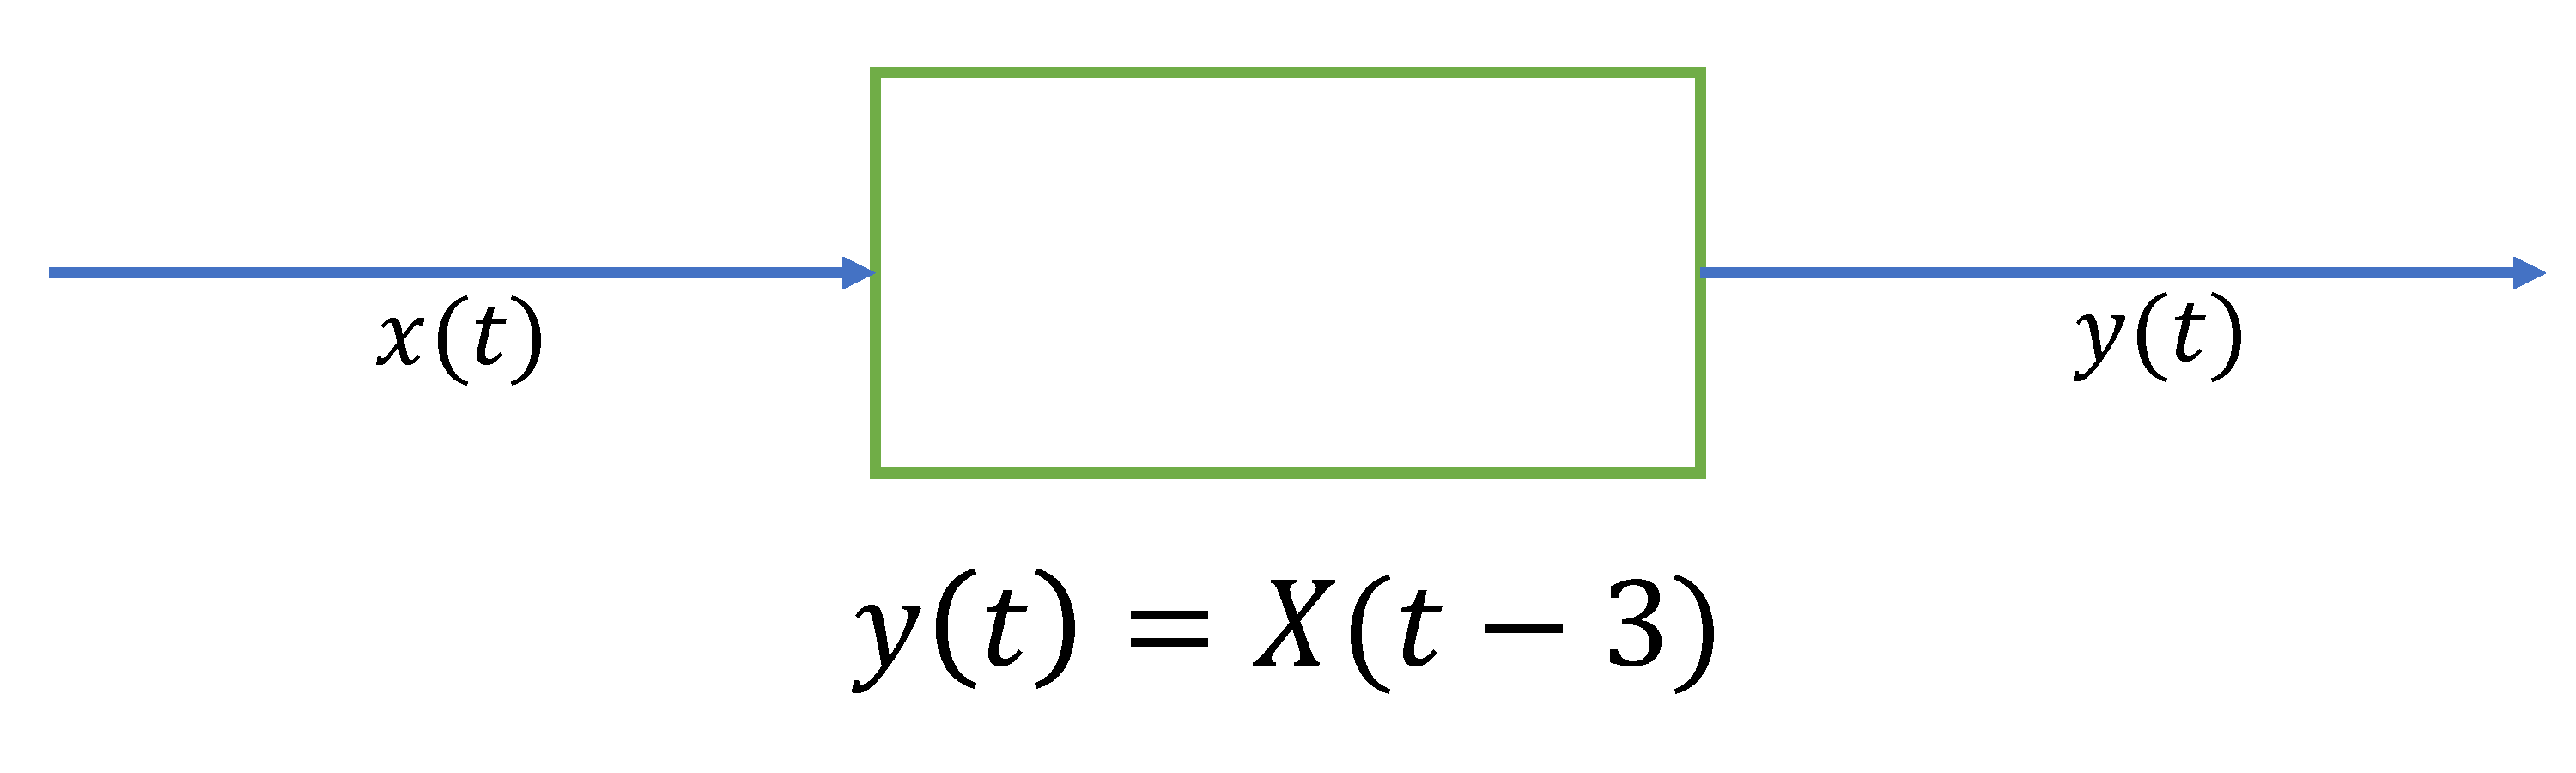
\includegraphics[width=120mm]{_20Q.pdf}
%\end{figure}
%}
%{حافظه دار است.}
%{خطی است.}
%{غیرعلی است.}
%{تغییر ناپذیر در زمان است.}
%%%%%%%%%%%%%%%%%%%%%%%%%%%%%%
%\test{
%سیگنال $x(t)$ که دارای تبدیل فوریه‌ای با اندازه و فاز زیر است کدام است؟
%\begin{figure}[h!]
%\centering
%\begin{subfigure}{0.49\textwidth}
%\includegraphics[width=80mm]{_21Q_ab.eps}
%\end{subfigure}
%\begin{subfigure}{0.49\textwidth}
%\includegraphics[width=80mm]{_21Q_an.eps}
%\end{subfigure}
%\end{figure}
%}
%{${3\over \pi t^2}(3\pi t\cos 3\pi t-\sin 3\pi t)$}
%{${3\over \pi t}(3\pi t\sin 3\pi t-\cos 3\pi t)$}
%{$3\sin 3\pi t\over \pi t^2$}
%{$3\cos (3\pi t+{\pi\over 4})\over \pi t^2$}
%%%%%%%%%%%%%%%%%%%%%%%%%%%%%%
%\test{
%ورودی یک سیستم LTI 
%$
%x(t)=\cos 100\pi t [u(t)-u(t-5)]
%$
% و پاسخ ضربه ی آن
%$
%h(t)=x(5-t)
%$
%است. مقدار خروجی در لحظه‌ی 
%$
%t=6
%$
%($y(6)$) چیست؟
%}
%{2}
%{$5\over 2$}
%{$9\over 2$}
%{5}
%%%%%%%%%%%%%%%%%%%%%%%%%%%%%%
%\test{
%$x[n]$
% یک سیگنال متناوب با دوره‌ی تناوب $N$ زوج است. اگر 
%$
%z[n]=x[2n]
%$
% و ضرایب سری فوریه‌ی 
%$
%x[n]
%$
% دارای خاصیت 
%$
%a_k=a_{k+{N\over 2}}
%$
% باشند، سیگنال 
%$
%x[2n+1]
%$
%کدام است؟
%}
%{$x[2n+1]=-z[n]$}
%{$x[2n+1]=(-1)^nz[n]$}
%{$x[2n+1]=0$}
%{$x[2n+1]=(-1)^n$}
%%%%%%%%%%%%%%%%%%%%%%%%%%%%%%
%\test{
%رابطه‌ی ورودی و خروجی در یک سیستم توسط رابطه‌ی زیر بیان می شود:
%$$
%y(t)=\begin{cases}
%x(t-1)&,\quad x(t-1)\le 1
%\\
%x(t-2)&,\quad x(t-1)> 1
%\end{cases}
%$$
%این سیستم کدام خواص زیر را دارد؟
%}
%{علی و خطی}
%{علی و غیرخطی}
%{غیرعلی و خطی}
%{غیرعلی و غیرخطی}
%%%%%%%%%%%%%%%%%%%%%%%%%%%%
%\testo{
%در هر مورد، سیگنال زمانی به همراه نرخ نمونه برداری متناظر آن داده شده است. در کدام گزینه، شرط نایکوئیست رعایت \underline{نمی شود}؟
%}
%{$x(t)={\sin \pi t\over \pi t}\ \ , \ \ F_s=1.2\text{ Hz}$}
%{$x(t)={\sin^2 \pi t\over (\pi t)^2}\ \ ,\ \ F_s=1.2\text{ Hz}$}
%{$x(t)=\sin 3t\ \,\ \ F_s={4\over \pi}\text{ Hz}$}
%{$x(t)={\sin \pi t\over \pi t}*e^{-|t|}\ \ ,\ \ F_s=3\text{ Hz}$
%که منظور از $*$ عملگر کانولوشن است.
%}
%%%%%%%%%%%%%%%%%%%%%%%%%%%%
%\test{
%تبدیل فوریه‌ی کدام یک از سیگنال های داده شده‌، دارای همه‌ی ویژگی‌های زیر است؟
%
%الف) 
%$
%\Re\{X(j\omega)\}=0
%$
%
%ب)
%$
%\int_{-\infty}^\infty \omega X(j\omega) d\omega=0
%$
%
%پ)
%$
%\int_{-\infty}^\infty X(j\omega) d\omega=0
%$
%}
%{$x(t)=e^{-t^2}-1$}
%{$x(t)=t^2e^{-|t|}$}
%{$x(t)=t^3e^{-|t|}$}
%{$x(t)=te^{-|t|}$}
%%%%%%%%%%%%%%%%%%%%%%%%%%%%%%
%\test{
%اگر سیگنال 
%$
%x(t)
%$
% مانند شکل زیر باشد،
%\picnocapt{m_1Q.eps}{60mm}
% سیگنال 
%$
%x(-{t\over 2}-3)
%$
% کدام است؟
%}
%{\includegraphics[width=60mm]{m_1Q_opt1.eps}}
%{\includegraphics[width=60mm]{m_1Q_opt2.eps}}
%{\includegraphics[width=60mm]{m_1Q_opt3.eps}}
%{\includegraphics[width=60mm]{m_1Q_opt4.eps}}
%%%%%%%%%%%%%%%%%%%%%%%%%%%%%%%
%\test{
%ضرایب سری فوریه‌ی سیگنال متناوب 
%$
%x[n]
%$
% با دوره تناوب 6 را با 
%$
%\alpha_k
%$
% نمایش می‌دهیم. از روی سیگنال 
%$
%x[n]
%$
%، سیگنال 
%$
%s(t)
%$
% را به صورت 
%$
%s(t)=\sum_{k=-\infty}^{\infty}x[k]\delta(t-2k)
%$
% می‌سازیم. ضرایب سری فوریه‌ی 
%$
%s(t)
%$
% کدام است؟
%}
%{${1\over 2}\alpha_k$}
%{${1\over 6}\alpha_k$}
%{$6\alpha_k$}
%{$2\alpha_k$}
%%%%%%%%%%%%%%%%%%%%%%%%%%%%%%%
%\test{
%اگر سیگنال 
%$
%x(4-2t)
%$
% مانند شکل زیر باشد،
%\picnocapt{m_2Q.eps}{60mm}
% سیگنال 
%$
%x(t)
%$
% کدام است؟
%}
%{\includegraphics[width=60mm]{m_2Q_opt1.eps}}
%{\includegraphics[width=60mm]{m_2Q_opt2.eps}}
%{\includegraphics[width=60mm]{m_2Q_opt3.eps}}
%{\includegraphics[width=60mm]{m_2Q_opt4.eps}}
\end{document}